\chapter{Daten Akquisition}
\markright{\thechapter \,\,\currentname \, - Philipp Kappus}
\label{chap:akquisition}
Jede*r Nutzer*in, der die Dienste von Twitter benutzen will, kann dies nur nach Bestätigung der allgemeinen Geschäftsbedingung tun. Damit erteilt ein*e Nutzer*in Twitter die Erlaubnis "`Ihre Inhalte weltweit verfügbar zu machen und dies auch Dritten zu ermöglichen" '\cite[Absatz 3]{twitter-agb}
Diese Bedingung bietet Twitter die Möglichkeit veröffentliche Tweets für Dritte (Unternehmen, Organisationen oder Einzelpersonen) über eine \ac{API} bereitzustellen und zu verkaufen. Im Folgenden wird beschrieben wie diese \ac{API} genutzt wurde um eine Datenbasis an Tweets zu erhalten.\\

\section{Tweets sammeln}
\label{sec:tweets-sammeln}
Tweets die in der Vergangheit veröffentlicht wurden, können über die sogenannte "`Search API"' angefordert werden. Um die Suche einzugrenzen kann die Sprache der Tweets und im Text vorkommende Wörter sowie ein Zeitraum definiert werden. 
Konstenlos stellt Twitter die Daten der letzten 7 Tage zur Verfügung; durch eine Hochrechnung wurde das genutzt um eine Größenabschätzung der Anzahl an Tweets zu erhalten die monatlich zur Thema der Covid-19 Pandemie veröffentlicht werden.
So konnte eine Gesamtheit von \textit{ca. 1.500.000} Tweets geschätzt werden. 
Um diese Methode in die Vergangheit zu erweitern bedarf es den sogenannten "`Full-Archive"' - Zugriff, der 1899\$ für 1.250.000 Tweets pro Monat kosten. Mit dem verfügbaren Budget der Arbeit war dies nicht zu realisieren.\\ \newline
Neben dem Zugriff auf in der Vergangheit veröffentlichte Tweets, bietet Twitter außerdem die Möglichkeit in Echtzeit (sobald er veröffentlicht wurde) jeden Tweet zu erhalten, wenn er vom Entwickler definierten Kriterien erfüllt.
Dieser Dienst steht konstenlos zur Verfügung.
Es wurde sich auf den sogenannte "`Filtered Stream"' mit den Kritieren: 1. Ein Tweet soll das Schlagwort "`Corona"' oder "`Covid"' (und damit auch "`Covid-19"') und 2. Der Tweet muss in deutscher Sprache verfasst sein, registiert um kontinuierlich jeden Tweet zu erhalten, der mit diesen Kriterien veröffentlicht wird. \\ \newline
Die gesammelten Tweets sollen nun in einer Datenbank gesichert werden. 
Für die Implementierung wurde \ac{AWS} genutzt. Eine \gls{EC2 - Instanz} ist für die Registeriung an der Twitter API und das Weiterleiten der Tweets verantwortlich. Als Speichermedium wurden \glspl{S3 - Bucket} verwendet. Um bei einem erhöhten Datenaufkommen keine Daten zu verlieren wurde zwischen die \gls{EC2 - Instanz} und den \glspl{S3 - Bucket} ein \gls{Amazon Kinesis Data Firehose} geschaltet, der sich durch eine hohe Datenaufnahme kennzeichnet. 
Dieser sammelt die einzelnen Tweets, fügt ca. 20 - 30 davon in einer Datei zusammen und speichert sie in den \glspl{S3 - Bucket} ab. 
Die Ordnerstruktur baut sich nach dem Zeitpunkt des Speicherns auf: \textit{Jahr/Monat/Tag/Stunde/}.
Eine Übersicht über die Architektur ist in Abbildung \ref{fig:aws-architecture} gegeben.
\begin{figure}[h]
	\centering
	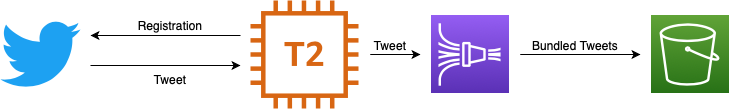
\includegraphics[width=0.7\linewidth]{images/AWS-architecture}
	\caption{\ac{AWS} - Architektur zur Tweet Akquisition}
	\label{fig:aws-architecture}
\end{figure}

Der Prozess lief 5 Monate vom 01.12.2020 bis zum 30.04.2021. 
Dadurch konnten insgesamt ca. 10.000.000 Tweets gesammelt werden, also ca. 2.000.000 Tweets pro Monat.

\section{Struktur eines Tweets}
\label{sec:struktur-eines-tweets}
Ein Tweet ist ein \ac{JSON} - Objekt, dass folgende, für die Arbeit relevanten, Informationen enthält:
\begin{enumerate}
	\item Der Zeitpunkt, an dem dieser Tweet veröffentlicht wurde
	\item Eine eindeutige Nummer, die diesen Tweet identifiziert
	\item Eine Liste an verwendeten \glspl{Hashtag}
	\item Informationen über den/die Nutzer*in der/die diesen Tweet veröffentlicht hat: 
	\begin{itemize}
		\item Eine eindeutige Nummer die diese*n Nutzer*in identifiziert
		\item Ein einzigartiger gewählte Nutzername
	\end{itemize}
	\item Ist ein Tweet ein \gls{Retweet}, so enthält dieser das komplette Tweet-Objekt des Original-Tweet.
\end{enumerate}



 